First we run a normal wordcount job on the cluster and use Memmetric to monitor it. In this wordcount job, no memory is used for storage therefore a presumable result would be a straight line close to the x-axis in the real-time monitor. However, the running result is shown in Fig. \ref{ref:baseline.png}.
\begin{figure}[ht]
  \centering
    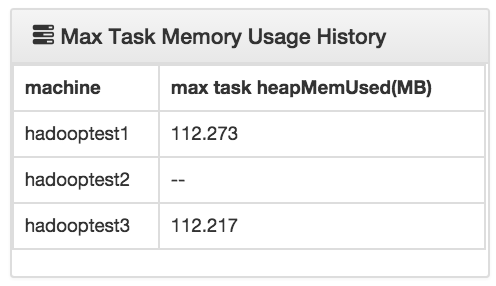
\includegraphics[width=2.1in]{image/baseline.png}
    \caption{Historical memory usage of normal wordcount job.}
    \label{ref:baseline.png}
\end{figure}